\documentclass[12pt]{article}
\usepackage{verbatim}
\usepackage{amsmath}
\usepackage{amssymb}
\usepackage{graphicx}
\usepackage[english]{babel}
\usepackage{caption}
\usepackage{subcaption}
\usepackage{ulem}
\usepackage{hyperref}

\usepackage{fullpage}
\usepackage{parskip}

\usepackage{amsmath,tikz}
\usetikzlibrary{shapes.geometric,arrows,positioning,calc}


%%% ------- New commands -------- %%%
\newcommand{\PoA}{\text{PoA}}

%%% ------- Game Pic ------- %%%%

\tikzstyle{player} = [draw, fill=red!80, shape=circle, minimum width=.25cm]
\tikzstyle{terminal} = [draw, shape = rectangle, fill=red!60, minimum width=.75cm, minimum height=.75cm]

%%% ------- Simulation ------- %%%%

\tikzstyle{Process} = [draw, shape = rectangle, fill=blue!20, minimum width=2.5cm, minimum height=1cm, text width=1.5cm,align=center]

\tikzstyle{Terminal} = [draw, fill=red!60,thick ,rectangle ,rounded corners, minimum width=3cm, minimum height=1cm]

\tikzstyle{Decision} = [draw, diamond ,minimum width=3.5cm, minimum height=1.5cm]

\tikzstyle{Result} = [draw , shape = rectangle, minimum width=1.5cm, minimum height=.8cm]

\tikzstyle{Arrow} = [->, >=latex', shorten >=1pt, thick]

\tikzstyle{left} = [draw, -latex',thick]

\title{Understanding the effect of selfish behaviour in a series of two queues.}
\author{Jason Young, Vincent Knight}

\begin{document}

\maketitle

\begin{abstract}

Healthcare systems and other queueing systems are often a series of complex queueing networks.
The best designed network can exhibit sub-optimal behaviour if the users of the system act rationally.
This is a basic idea underlying Game Theory.


There is a vast quantity of literature understanding this inefficiency which can be measured using a game theoretical measure entitled: Price of Anarchy (PoA).
However, most of the corresponding work concentrates on queues in isolation and/or in parallel.

In this paper two queues are considered in series.
The decisions of customers at the entry to both queues thus has an impact on the efficiency of the entire system.

\end{abstract}

% Keywords: Hierarchical queues in HC; PoA; Simulation model; Heuristics developed to obtain optimal policies;

\section{Introduction}\label{Introduction}

What damage do the selfish choices of some afflict onto the welfare of all?
The work presented in this paper answers this question in the context of queues in series.

There is a substantial quantity of literature on the subject of equilibrium behaviour of a queueing system where congestion is a factor influencing behaviour \cite{bell1983individual,chr1972individual,  edelson1971congestion, luski1976partial, naor1969regulation, yechiali1972customers}.
This can be traced back to a set of short communications between Leeman \cite{leeman1964reduction, leeman1965letter} and Saaty \cite{saaty1965burdens}.

This paper builds on this literature by considering a particular network of queues.
For most public services, congestion is a negative aspect of service quality.
When leaving one queue; customers (which we will refer to as players) often join a second queue and this is what is referred to as a hierarchical queueing system (as shown in Figure \ref{game_pic}).

The following is a general conclusion of a majority of the literature:

\begin{center}
\textit{Selfish users make busier systems.}
\end{center}

Naor cites the initial exchange between Leeman and Saaty as the motivation for his early work on queuing systems.
In \cite{naor1969regulation}, thresholds are obtained that give the number of players $\tilde n$ at which selfish users should ``balk'' a particular queue.
Furthermore, a threshold $n^*$ is obtained that ensures average optimal utility.

In \cite{bell1983individual}, similar work is carried out for multiple $M/M/1$ queues in parallel where players chose which queue to join.
Importantly, this work differs from \cite{naor1969regulation} in that it considers ``unobservable'' queues.

In \cite{knight2012comparisons}, results are given regarding the comparison of observable and unobservable approaches.

A good review of the mentioned works and further pieces of literature is found in \cite{hassin2003queue}.

The effect of selfish behaviour when compared to optimal behaviour in game theoretical contexts is measured as the ``Price of Anarchy'' (PoA) \cite{koutsoupias2009worst, roughgarden2002bad}.
This is defined as the ratio of the selfish ($\tilde C$) and optimal ($C^*$) costs:

$$
\PoA = \frac{\tilde C}{C^*}
$$

In \cite{knight2013selfish} the PoA is calculated for a healthcare system.
Patient choices between hospitals are considered as $M/M/c$ queues in parallel.

The contribution of this paper is to consider two stations (to avoid confusion we will refer to a queue and service station as a station) in series allowing for two consecutive decisions: whether or not to join the station.
Players who join the first station upon completion of service will potentially drop out from the entire system.
A potential application of this is a healthcare system where patients must choose to see their general practitioner before obtaining care from a specialist/emergency centre.
If unable to get an appointment within a short enough period of time, patients may choose to go directly to their specialist/emergency centre \cite{Mail_millions}.

In Section \ref{model}, the model will be described.
A novel aspect of this work is that the cost of a given policy is evaluated through the use of purpose built Agent Based Simulation (ABS).
In Section \ref{heuristicoptimalpolicies} various heuristic approaches to obtaining optimal policies are considered.
These range from random search algorithms to a more sophisticated approach that depends on the analytical formula for an $M/M/c$ queue \cite{stewart2009probability}.
Before concluding in Section \ref{conclusions} a variety of numerical experiments will be shown in Section \ref{results} demonstrating the effect of selfish decision making in queues in series.

\section{Model}\label{model}

Let $k\in\{1,2\}$ be the index for each station in the system.
The players arrive into the system at a rate $\Lambda$.
Upon arriving at the station $k$ players are aware of:

\begin{itemize}
    \item The service rate $\mu_k$;
    \item The number of servers $c_k$;
    \item The number of players already at station $k$: $m_k$;
    \item The skip cost of station $k$: $\beta_k$.
\end{itemize}

Upon observing a station, players must select one of two potential strategies: `join' or `skip'.
The strategy picked at station $k$ is denoted by $d_k\in\{0,1\}$:

\begin{equation}\label{eq:decision}
    d_k=
\begin{cases}
    1,& \text{if player joins queue } k \\
    0,& \text{if player skips queue } k
\end{cases}
\end{equation}

The cost associated with joining station $k$ is denoted by $J_k$ and corresponds to the actual time spent in station $k$.
The cost associated with skipping station $k$ is denoted by $\beta_k$.
This cost is measured in units of time but is a constant value to be interpreted as the ``value of service'' at station $k$.
The cumulative cost of going through the entire system is given by $C=C(d)=C_1(d)+C_2(d)$ where:

\begin{equation}\label{eq:actualcost}
C_{k} = \begin{cases}
        \beta_k&\text{if }d_k=0\\
        J_k&\text{if }d_k=1\\
        \end{cases}
\end{equation}

The expected value of $J_k$ when there are $m_k$ players present upon arrival in system $k$ is given by:

\begin{equation} \label{eq:expect}
	E[J_{k}] = \frac{m_k+1}{\mu_k c_k}
\end{equation}

A final parameter of our model is the dropout probability $p$.
This is the probability with which a player who joins the first station will exit the entire system (implying $C_2=0$).

All of this is summarised in Figure \ref{game_pic}.

\begin{figure}[!hpbt]
\begin{center}
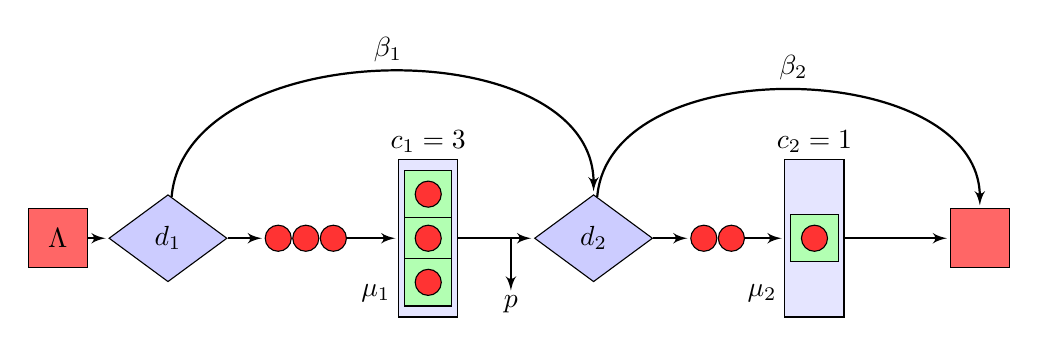
\begin{tikzpicture}[scale=.7]
            \draw (0,0) node[terminal] (A) {};
            \node (B) [diamond, fill=blue!20, draw, minimum width=1.5cm, minimum height=1cm] at (2, 0) {$d_1$};
            %%%%% First station %%%%%
            \draw (4,0) node[player] (C) {};
            \draw (4.5,0) node[player] (Q) {};
            \draw (5,0) node[player] (D) {};
            \draw [Arrow] (A) -- (B);
            \draw [Arrow] (B) -- (C);
            \node (E) [rectangle, fill=blue!10, draw, minimum width=.75cm, minimum height=2cm, right=1.0cm of Q] {};
            \draw [Arrow] (D) -- (E);
            \node (F) [rectangle, fill=green!30, draw, minimum width=.6cm, minimum height=.6cm] at (E) {};
            \node (G) [rectangle, fill=green!30, draw, minimum width=.6cm, minimum height=.6cm] at ($(E) + (0,.8)$) {};
            \node (H) [rectangle, fill=green!30, draw, minimum width=.6cm, minimum height=.6cm] at ($(E) + (0,-.8)$) {};
            \draw node[player] at (F) {};
            \draw node[player] at (G) {};
            \draw node[player] at (H) {};
            \node at ($(E) + (0,1.75)$) {$c_1=3$};
            \node at ($(E) + (-.95,-1)$) {$\mu_1$};
            %%%%% Second station %%%%%

            \node (Z) [diamond, fill=blue!20, draw, minimum width=1.5cm, minimum height=1cm] at ($(E) + (3,0)$) {$d_2$};

%            \node (R) [diamond, fill=blue!20, draw, minimum width=1.5cm, minimum height=1cm] at ($(Z) + (3,0)$) {$d_n$};
            \draw [Arrow] (E) -- (Z);
            \draw node[player] (I) at ($(Z) + (2,0)$) {};
            \draw node[player] (J) at ($(I) + (.5,0)$) {};
            \node (K) [rectangle, fill=blue!10, draw, minimum width=.75cm, minimum height=2cm, right=.5cm of J] {};
            \draw [Arrow] (Z) -- (I);
            \draw [Arrow] (J) -- (K);
            \node (L) [rectangle, fill=green!30, draw, minimum width=.6cm, minimum height=.6cm] at (K) {};
            \draw node[player] at (L) {};
            %%%%% End station %%%%
            \node (M) [terminal] at ($(K) + (3,0)$) {};
            \draw [Arrow] (K) -- (M);
            %%%%% Edges %%%%%
            \draw (Z) edge[out=85,in=90,Arrow] node [above] {$\beta_2$} (M);
            \draw (B) edge[out=85,in=90,Arrow] node [above] {$\beta_1$} (Z);
            \node at ($(K) + (0,1.75)$) {$c_2=1$};
            \node at ($(K) + (-.95,-1)$) {$\mu_2$};
            \node at (A) {$\Lambda$};

            %%%%% Dropout probability %%%%
            \draw ($(Z) !.5! (E)$) edge[Arrow] node [below = .25cm] {$p$} ($(Z) !.5! (E) + (0,-1)$);

        \end{tikzpicture}
    \end{center}

    \caption{Diagrammatic representation of the model.}
	\label{game_pic}

\end{figure}

If a general population of players is considered a state dependent policy $\tau = (n_1, n_2)$ can be defined that all players follow.
In general this policy will be of the form:

$$d_k = \begin{cases}
1,& \text{if }m_k\leq n_k\\
0,&\text{ otherwise}
\end{cases}$$

Where $m_k$ is the number of players present at station $k$ upon having to make a decision $d_k$.
In other words a policy $\tau$ is a set of two threshold policies, one for each station, simply denoting a threshold at which players skip.
As $d=d(\tau)$ we have $C=C(\tau)$.


\subsection{Simulation engine}

To evaluate the $C(\tau)$ for given $\tau$ a bespoke simulation model has been developed  (written in Python \url{http://www.python.org/}).
The model itself is a combination of Discrete Event and Agent Based Simulation (taking advantage of the Object Orientated framework available in Python) \cite{robinson2004simulation}.
The flow of the simulation model is shown in Figure \ref{fig:Simflow}.

\begin{figure}[!hbpt]

        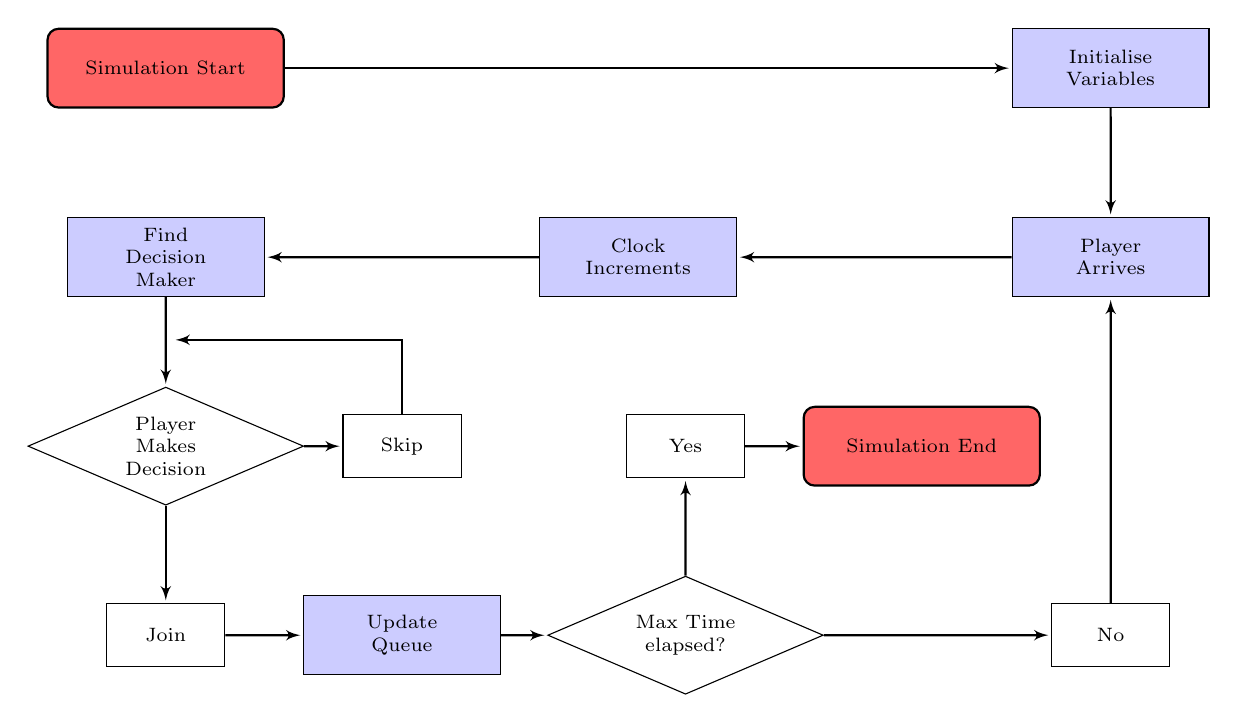
\begin{tikzpicture}[scale=.6]
        \tikzstyle{every node} = [font=\scriptsize ]

        %%%%% Top Line %%%%%%

        \draw (0,0) node[Terminal] (A) {Simulation Start};
        \draw node[Process] at ($(A)+ (20,0)$) (B) {Initialise Variables};


        %%%%% Second Line %%%%%

        \draw node[Process] at ($(B)+ (0,-4)$) (C){Player Arrives};
        \draw node[Process] at ($(C)+ (-10,0)$) (D){Clock Increments};
        \draw node[Process] at ($(D)+ (-10,0)$) (E){Find Decision Maker};

        %%%%% Third Line %%%%%

        \draw node[Decision] at ($(E) + (0,-4)$) (F){};
        \node[text width=1.5cm,align=center] at (F) {Player Makes  Decision};
        \draw node[Result] at ($(F) + (5,0)$) (G){Skip};
        \draw node[Result] at ($(G) + (6,0)$) (H){Yes};
        \draw node[Terminal] at ($(H) + (5,0)$) (I){Simulation End};

        %%%%% Bottom Line %%%%%

        \draw node[Result] at ($(F)+ (0,-4)$) (J){Join};
        \draw node[Process] at ($(J) + (5,0)$) (K){Update Queue};
        \draw node[Decision] at ($(H) + (0,-4)$) (L){};
        \node[text width=1.5cm,align=center] at (L) {Max Time elapsed?};
        \draw node[Result] at ($(C) + (0,-8)$) (M){No};

        %%%%% Connecting Arrows %%%%%

        \draw [Arrow] (A) -- (B);
        \draw [Arrow] (B) -- (C);
        \draw [Arrow] (C) -- (D);
        \draw [Arrow] (D) -- (E);
        \draw [Arrow] (E) -- (F);
        \draw [Arrow] (F) -- (J);
        \draw [Arrow] (J) -- (K);
        \draw [Arrow] (K) -- (L);
        \draw [Arrow] (L) -- (M);
        \draw [Arrow] (M) -- (C);
        \draw [Arrow] (F) -- (G);
        \draw [Arrow] (L) -- (H);
        \draw [Arrow] (H) -- (I);

        \node[draw=none,fill=none] at ($(E)+ (0,-1.75)$) (dummy){};

        \path [left] (G.north) |- (dummy.east);

	\end{tikzpicture}

	\caption{Flow chart describing the simulation model}
	\label{fig:Simflow}
\end{figure}

The input to the model (apart from the system parameters described in Section \ref{model}) is a policy $\tau$ and the required output is $C(\tau)$.
An investigation of run time, warm up time, and number of trials was carried out to ensure a reliable value of $C(\tau)$ is output \cite{cite013}.
Graphical methods were used for system parameters discussed in Section \ref{results} and are shown in Figure \ref{runtime}.

\begin{figure}[!hbtp]
    $$\begin{array}{ccc}
        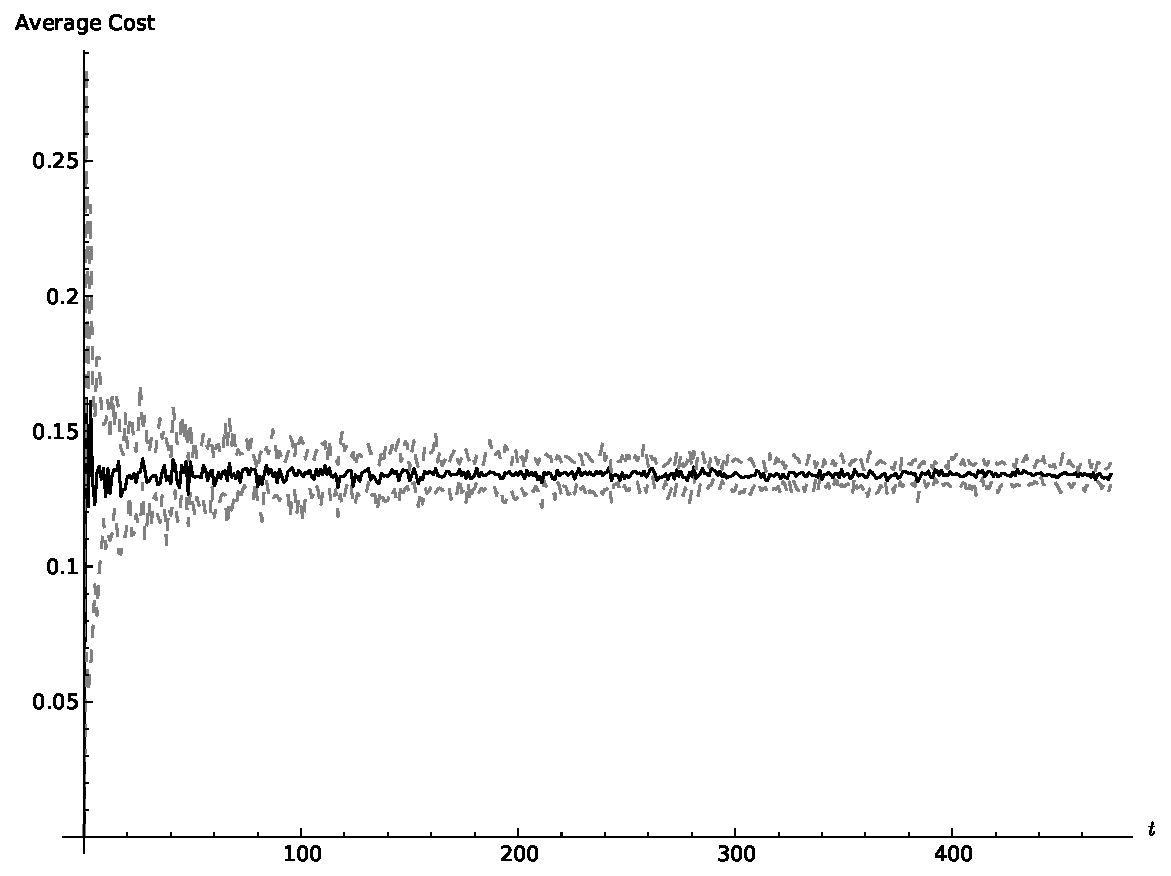
\includegraphics[width=.3\textwidth]{Images/Run_Time.pdf}&
        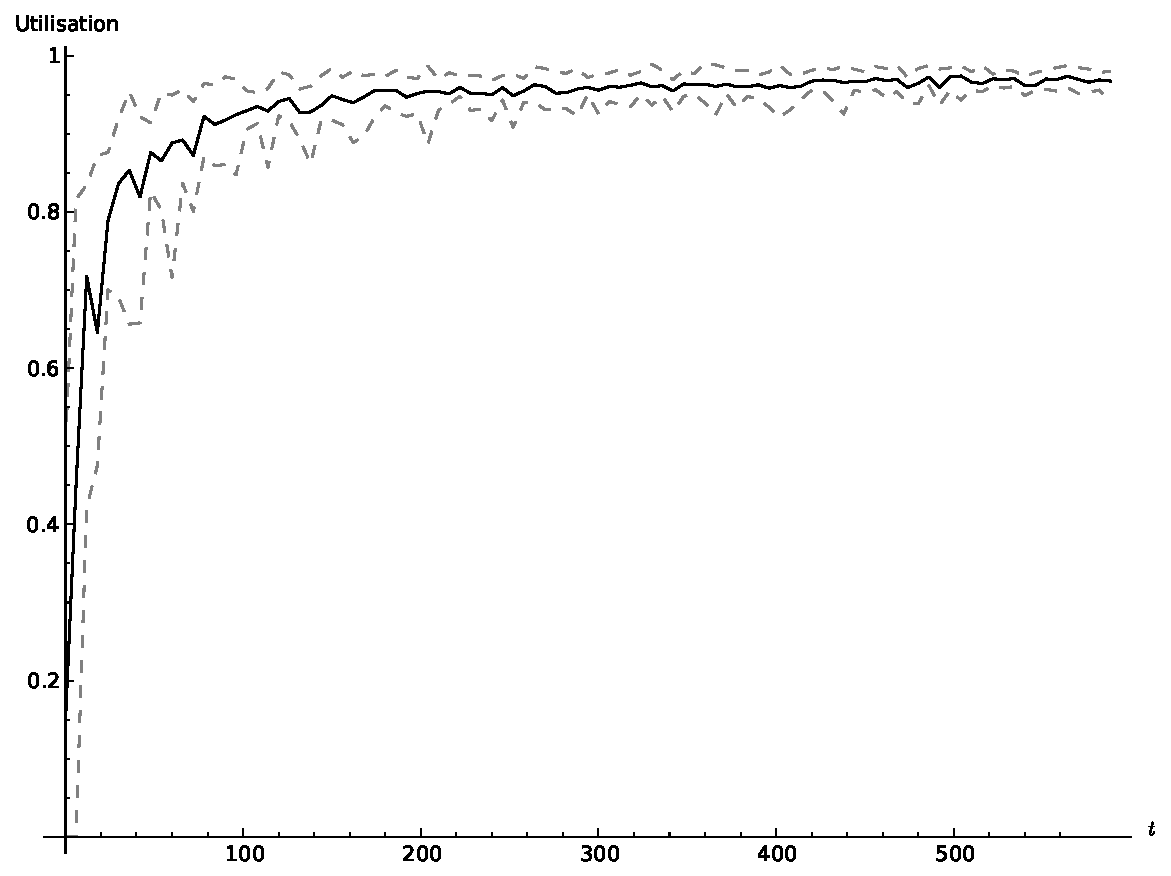
\includegraphics[width=.3\textwidth]{Images/Warm_up.pdf}&
        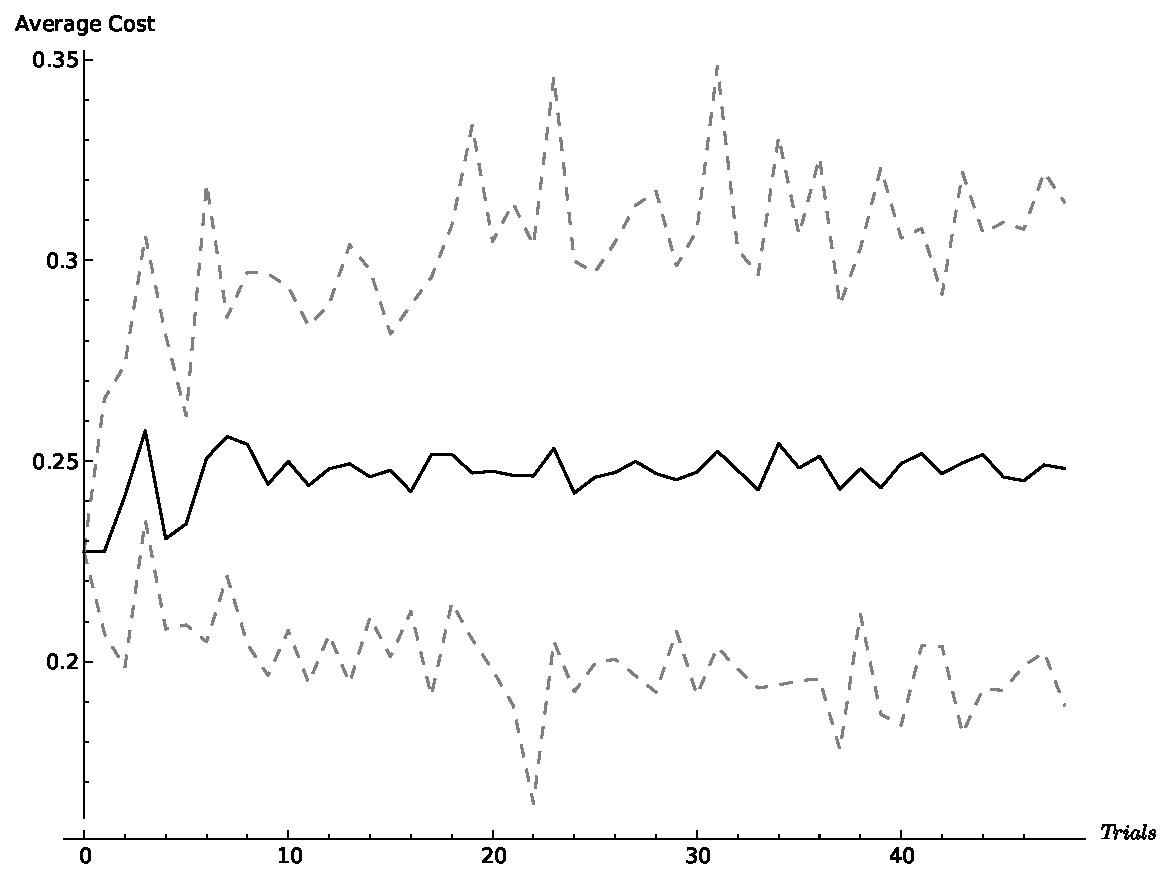
\includegraphics[width=.3\textwidth]{Images/Trials.pdf}\\
        \text{a: Run Time}& \text{b: Warm up time}& \text{c: Number of trials}
    \end{array}$$
    \caption{Investigating run time, warm up time and number of trials required to obtain reliable values of $C(\tau)$}\label{runtime}
\end{figure}

A run time of 250 time units was shown to reduce the variation in $C(\tau)$ (Figure \ref{runtime}a) whilst a warm up period of 50 time units reduced gave a stable utilisation of servers (Figure \ref{runtime}b).
Finally experiments of 16 trials each were chosen despite the lack of variation shown in Figure \ref{runtime}c.
This relatively large number of trials did not prove to be computationally expensive as they were all run in parallel using the Advanced Research Computing facilities at Cardiff University \url{http://www.cardiff.ac.uk/arcca/} (super computer).

\subsection{Selfish policy: $\tilde \tau$}

The selfish policy is the policy under which individual players reduce their expected cost.

To obtain the selfish policy an assumption is made: players are risk averse.
It is assumed that players ignore the dropout probability $p$ at station $1$ so that we have (recall equation (\ref{eq:decision})):

\begin{equation}\label{eq:selfishdecision}
    \tilde d_k=
\begin{cases}
    1,& \text{if } E[J_k] \leq \beta_k \\
    0,& \text{otherwise}
\end{cases}
\end{equation}

This in turn gives (recalling (\ref{eq:expect})):

\begin{equation}\label{eq:selfishpolicy}
\tilde\tau = \left(\lfloor\beta_1\mu_1 c_1 - 1\rfloor,\lfloor\beta_2\mu_2 c_2 - 1\rfloor\right)
\end{equation}


\subsection{Optimal policy: $\tau ^*$}

As discussed before, in general selfish users make busier system so that it seems reasonable to assume $n_k^*\leq \tilde n_k^*$ for $k\in\{1,2\}$.
A general result has in fact been shown confirming this for queues in parallel \cite{shone2014containment}.
However, this is not necessarily evident for queues in series with $p>0$.
Indeed, to reduce the mean value $C$ it is reasonable to assume that a gateway effect exists, where players are encouraged to join the first queue in order to exit the queue thanks to the dropout probability.
This is in fact readily understood in practice by policy makers: \cite{Mail_millions}.

Let $\Omega$ be the solution space to the optimisation problem of reducing the expected value of $C^*$:

\begin{equation}\label{searchspace}
\Omega = \left\{\tau=(n_1, n_2)\in\mathbb{Z}^2\;|\;0\leq n_1\leq 2\tilde n_1,\; 0\leq n_2\leq \tilde n_2 \right\}
\end{equation}

The optimal cost is thus defined as:

\begin{equation}\label{eq:optimal}
E[C^*]=\min_{\tau\in\Omega}E[C(\tau)]
\end{equation}

Note that the restriction of the optimisation problem to only consider stationary policies is potentially an incorrect one.
Indeed, a non homogeneous policy could in fact be optimal however considering dynamic programming techniques on the underlying Markov Decision process it can be seen that a threshold policy will in fact be optimal \cite{puterman2009markov}.

As discussed, the simulation model is used as an objective function for a given $\tau$.
In the next section, various heuristic approaches to obtaining $\tau^*$ (recall (\ref{eq:optimal}): this corresponds to the optimal policy) will be discussed.

\section{Heuristic Optimal Policies}\label{heuristicoptimalpolicies}

Using the simulation model as an objective function a variety of search based heuristics have been tested \cite{}. All of these use $\tilde\tau$ as an initial solution and make minor perturbations accepting improvements within a specific region:

\begin{itemize}
    \item Fixed search range: randomly evaluate a fixed range around the initial policy;
    \item Variable search range: increase the range of the search range;
    \item Random descent: randomly search the entire solution space;
    \item Iterative random descent: JASON CHECK THESE AND ALSO INCLUDE A SENTENCE FOR THIS ONE. I DONT LIKE THE NAMES. ARE THEY THE CORRECT NAMES?
\end{itemize}

\subsection{Heuristic 1}\label{heuristic1}

A comparison of the performance of the various heuristics above is shown in Figure \ref{basicsearch}.

\begin{figure}[!hbtp]
    \begin{center}
        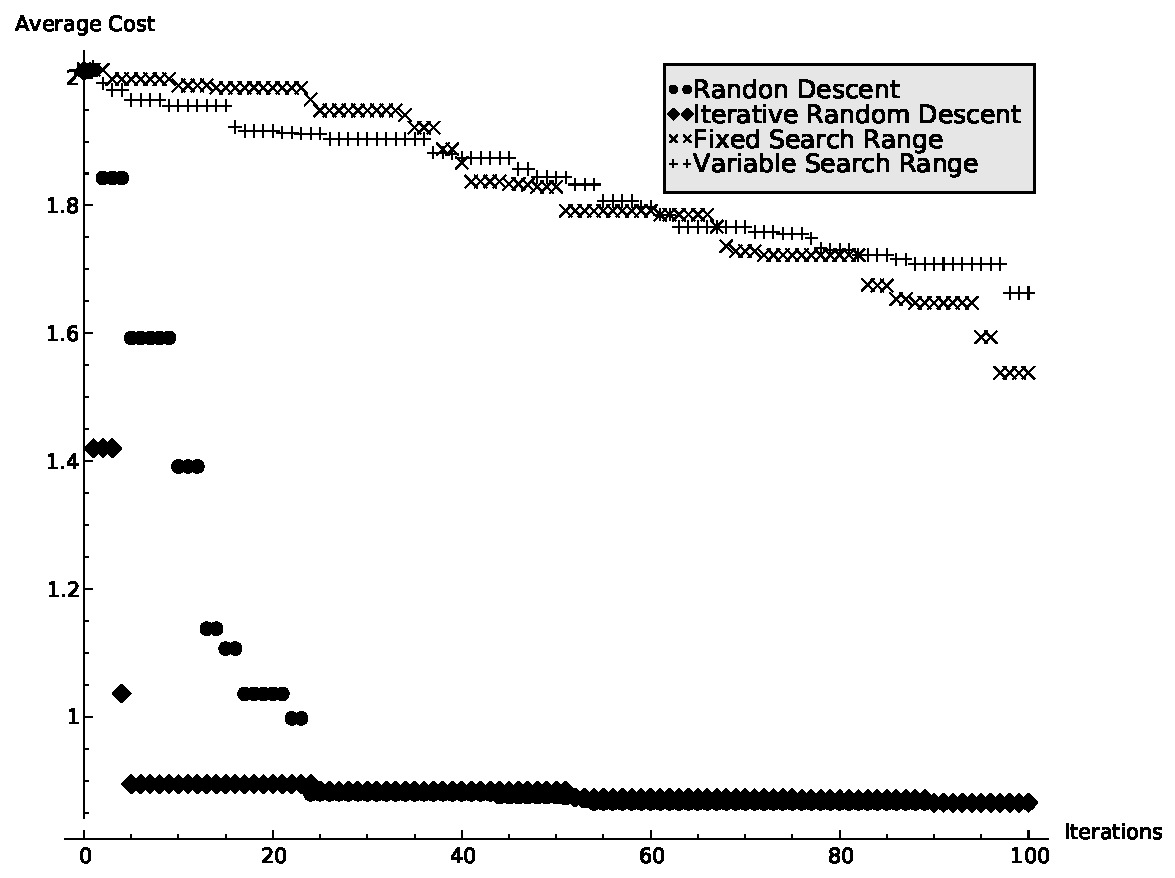
\includegraphics[width=.6\textwidth]{Images/Solver_Comp.pdf}
    \end{center}
    \caption{Comparing local search heuristics}\label{basicsearch}
\end{figure}

As shown, the most efficient of the chosen heuristics is the `Random Descent'.
This algorithm is nonetheless computationally expensive.
Some scenarios of Section \ref{results} taking various hours to run (despite the use of \cite{web002}).
The aim of the work presented here is to gain a global understanding of PoA behaviour and as such a large number of optimisations are needed.
The next sections will demonstrate further heuristics.

\subsection{Heuristic 2}\label{heuristic2}

This heuristic is based on the assumption that the arrival rate $\lambda_2$ at the second station is in fact Markovian.
For $p=0$ this is in fact not an assumption \ref{} however for $p>0$ the arrival rates at the second station no longer exhibit Markovian behaviour.
Nevertheless as shown in Figure \ref{casestudycomp} this heuristic performs very favourably and in fact the non Markovian behaviour seems to not affect the performance of our heuristic.

The arrival rate at the second station is given by:

\begin{equation}
\lambda_2 = \Lambda\times(1-p\times(1-\pi^{(1)}_{n_1}))
\end{equation}

Where $\tau=(n_1, n_2)$ and $\pi^{(1)}_{i}$ is the probability that the first station is in state $0\leq i\leq n_1$.
Note that the first station corresponds to an $M/M/c/n_1$ queue and so we have:

\begin{equation}\label{eq:probcl}
  \pi^{(1)}_i = \frac{1}{i!}\left(\frac{\Lambda}{\mu_1}\right)^{i}\pi_{0} \hspace{1cm} 0\leq i \leq c_i
\end{equation}

\begin{equation}\label{eq:probc_im}
  \pi^{(1)}_i = \frac{1}{c_i^{i-c_i}c_i!}\left(\frac{\Lambda}{\mu_1}\right)^{i}\pi_{0} \hspace{1cm} c_i< i \leq K
\end{equation}

where

\begin{equation}
\pi^{(1)}_{0} = \left[ \sum_{n=0}^{c_i-1} \frac{1}{n!} \left( \frac{\Lambda}{\mu_1} \right)^{n}  + \sum_{n=c_i}^{K} \frac{1}{c_i^{n-c_i}c_i!} \left( \frac{\Lambda}{\mu_1} \right)^{n} \right] ^{-1}
\end{equation}

Using the Markovian assumption as to the distribution of $\lambda_2$ a similar formula for $\pi_i^{(2)}$ can be obtained, replacing the relevant parameters.

Using this and recalling (\ref{actualcost}):

\begin{equation}\label{eq:ciapprox}
E[C_{i}] \approx \pi_{n_i}^{(i)} \beta_{i} + \sum_{j=0}^{c_{i}} \frac{\pi_{j}^{(i)}}{\mu_{i}} + \sum_{j=c_{i}}^{n_i-1}\frac{ \pi_{j}^{(i)}(j+1)}{ \mu_{i} c_{i}}
\end{equation}

and so:

\begin{equation}\label{eq:approxcost}
E[C]\approx E[C_1] + \frac{\lambda_2E[C_2]}{\Lambda}
\end{equation}

Note that the approximation of (\ref{eq:ciapprox}) is in fact an equality for $i=1$.
Using (\ref{eq:approxcost}) the cost of any policy $\tau$ can be approximated immediately and so $\tau^*$ can be heuristically obtained by an exhaustive search of the solution space.
To obtain an actual mean cost of $\tau^*$ the simulation model needs to only be run once.
A comparison of heuristics 1 and 2 is shown in Figure \ref{casestudycomp}, it is evident that the assumption made with regards to the Markovian nature of $\lambda_2$ do not seem to have a large effect.
The fact that results for $\Lambda >130$ are not shown for heuristic 1 are due to the fact that they were not obtained as they required more than 80 hours of computations on \cite{web002}.

\begin{figure}[!hbtp]
    \begin{center}
        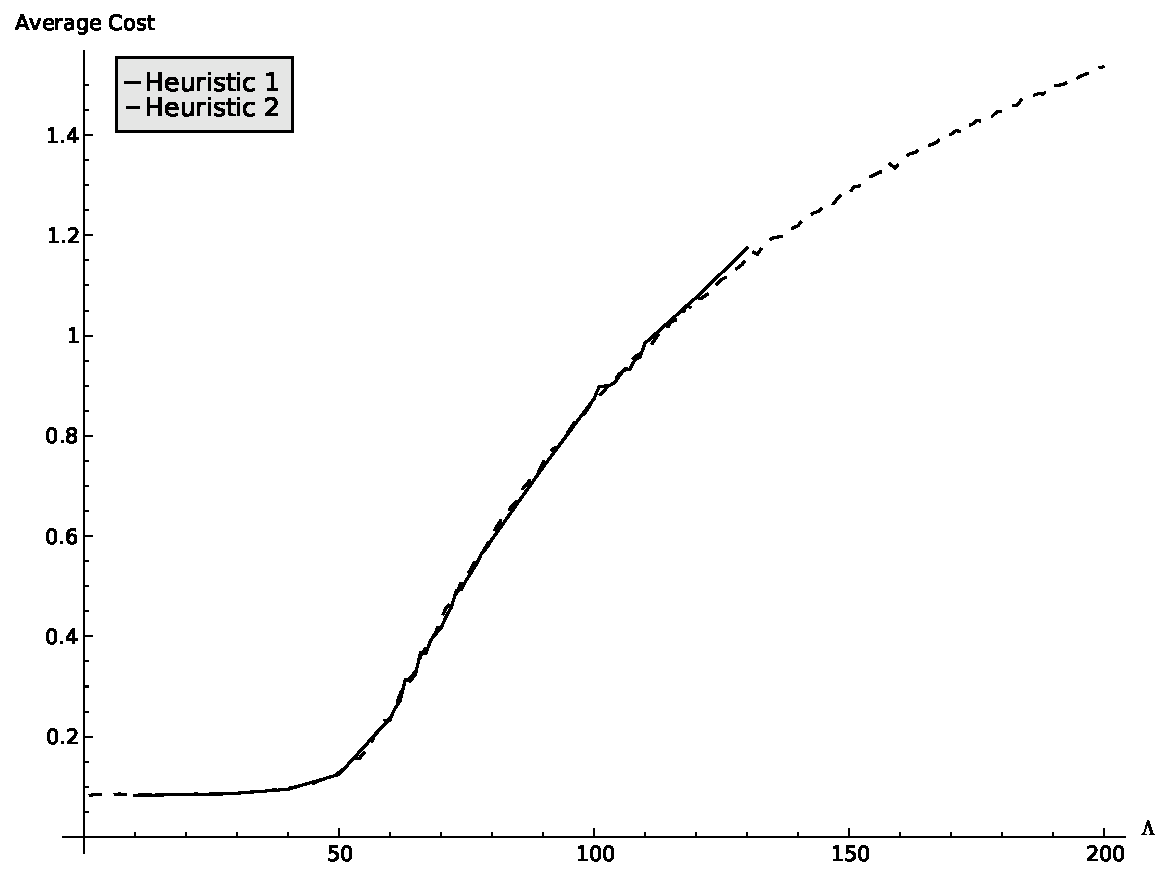
\includegraphics[width=.6\textwidth]{Images/CaseStudyComp.pdf}
    \end{center}
    \caption{Comparing Heuristic 1 and 2}\label{casestudycomp}
\end{figure}

Before considering various results in Section \ref{results}, one final heuristic is proposed that only applies if $c_1=c_2=1$.

\subsection{Heuristic 3}\label{heuristic3}

In \cite{Naor} thresholds $n^*$ are obtained for single server queues that optimise the expected cost. $n^*$ is shown to be the solution to the following inequality:

\begin{equation}\label{eq:naor}
  \leq  n ^ * \leq
\end{equation}

Using (\ref{eq:naor}) another potential policy is $\tau = (n^*_1, n^*_2)$.
Figure \ref{allheuristics} shows a comparison of these three heuristic approaches for a series of single server queues.

\begin{figure}[!hbtp]
    \begin{center}
        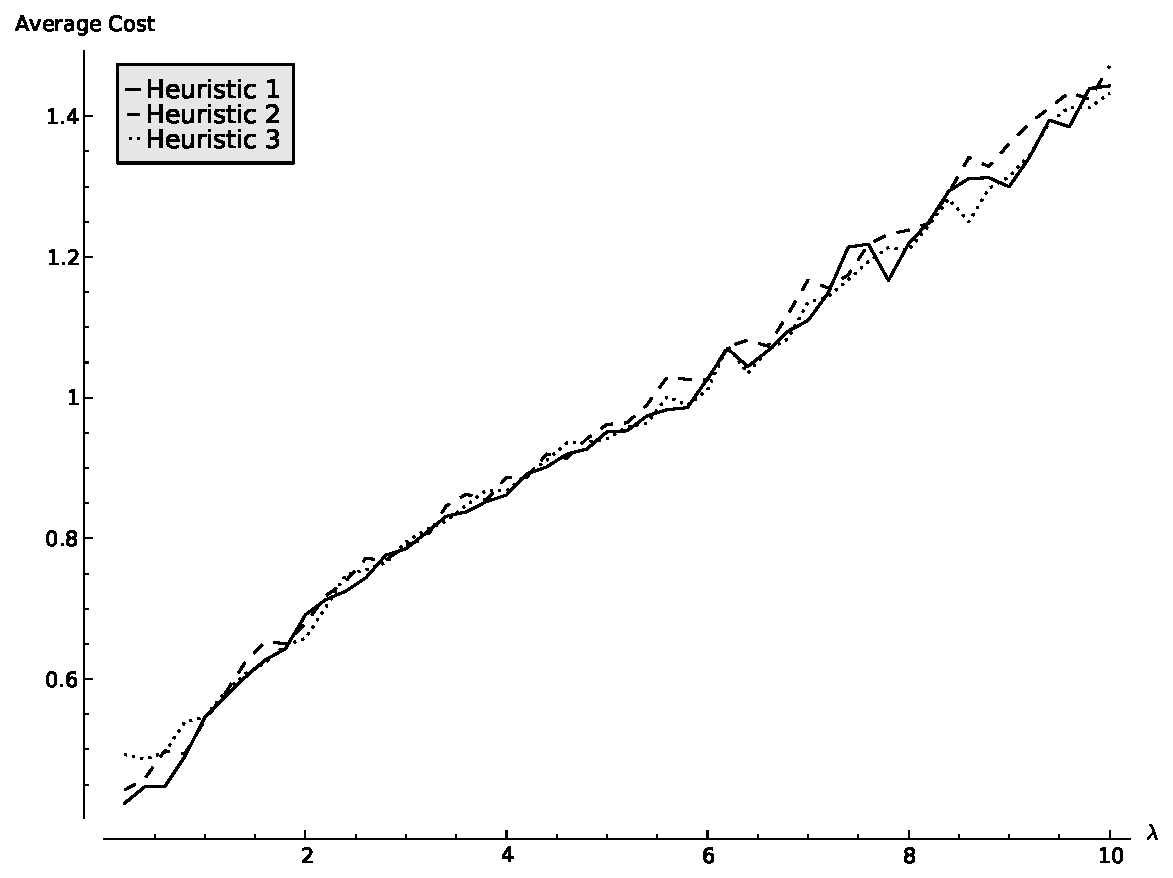
\includegraphics[width=.6\textwidth]{Images/Exit0.pdf}
    \end{center}
    \caption{Comparing all heuristics}\label{allheuristics}
\end{figure}

All the heuristics seem to behave adequately (this has been confirmed through a large quantity of experimentation).
For the purposes of this paper heuristic 2 will be used from now on given the very low computational cost.

\section{Results}\label{results}

As discussed in Section \label{introduction} an immediate application of the models developed is healthcare.
Using data from \cite{} we consider two stations in series:

\begin{itemize}
    \item A General practitioner with 5 servers each able to see 12.5 patients a day. Furthermore patients consider a wait of 2 days as acceptable to see their GP:

        $$c_1=5, \mu_1=12.5, \beta_1=2$$

    \item After seeing a GP or after deciding the wait to see a GP is too long \cite{FINDSOMEPOPNEWSABOUTTHIS} patients may choose to proceed to the Emergency Department (ED). It is assumed that the ED has a capacity of 5 servers each able to 2 patients an hour. An acceptable wait is now assumed to be 8 hours which is in line with national targets \cite{}.

        $$c_2=5, \mu_1=48, \beta_1=1/3$$
\end{itemize}

It is assumed that 80\% of patients who see their GP do not need to attend the ED:

$$p=.8$$

For these sets of parameters, using heuristic 2 a Price of Anarchy can be calculated.
For example for $\Lambda=?$ the PoA is 5 which implies that the overall patient utility is 5 times as bad when patients act selfishly.

Figure \ref{ana_lambda} shows the effect of $\Lambda$ on the PoA for different values of service ($\beta$).
The profile of this curve is very similar to profiles of curves seen in \cite{VKPH}.
For low demand the PoA is 1: this implies that the capacity of the system is sufficient to deal with the actions of selfish users.
As the demand increases, the first station starts to get congested.
Optimal behaviour will at this point encourage players to skip the first queue (before the expected wait reaches $\beta_1$.
Selfish users however will wait until the system becomes very busy before they are willing to start skipping.
This occurs when the demand increases further and we see an initial drop of the PoA.
Recall that this simply implies that selfish users are not causing the system to behave in a different way to the optimal behaviour.
This is something that has been noted in the literature: \cite{bunchofpapers}: in congested systems selfish users don't make a difference.
This is particularly relevant to healthcare where most healthcare systems are already severely over congested.

\begin{figure}[!hbtp]
    \begin{center}
        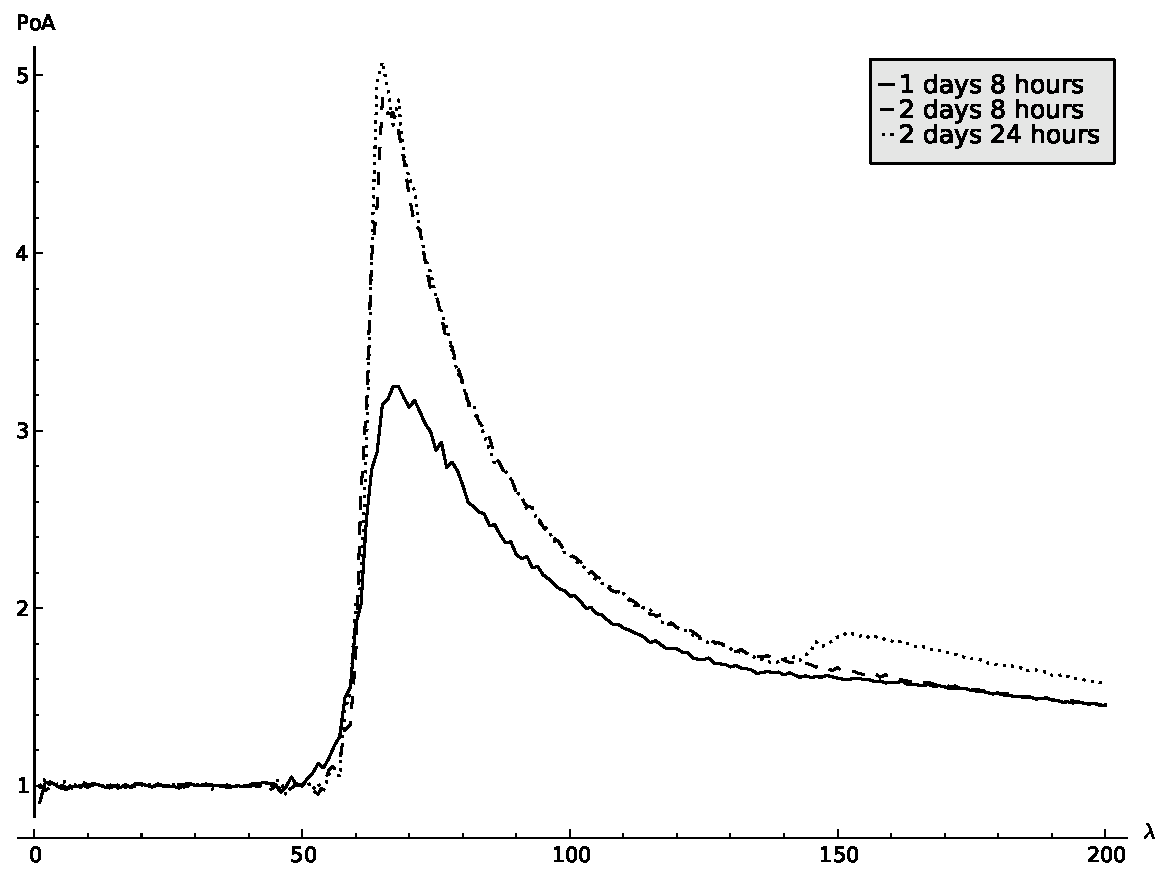
\includegraphics[width=.5\textwidth]{Images/Ana_Lambda.pdf}
    \end{center}
    \caption{PoA for varying lambda}\label{ana_lambda}
\end{figure}

Figure \ref{singlePoA} shows the PoA for both systems taken in isolation. BLABLABLA...

\begin{figure}[!hbtp]
    \begin{center}
        [Grab picture of PoA for both single stations]
    \end{center}
    \caption{PoA for varying lambda}\label{ana_lambda}
\end{figure}

The effect of having the two queues in series is...
Note that this is shown in Figure \ref{dualpeak} where GET PARAMETERS HERE.

\begin{figure}[!hbtp]
    \begin{center}
        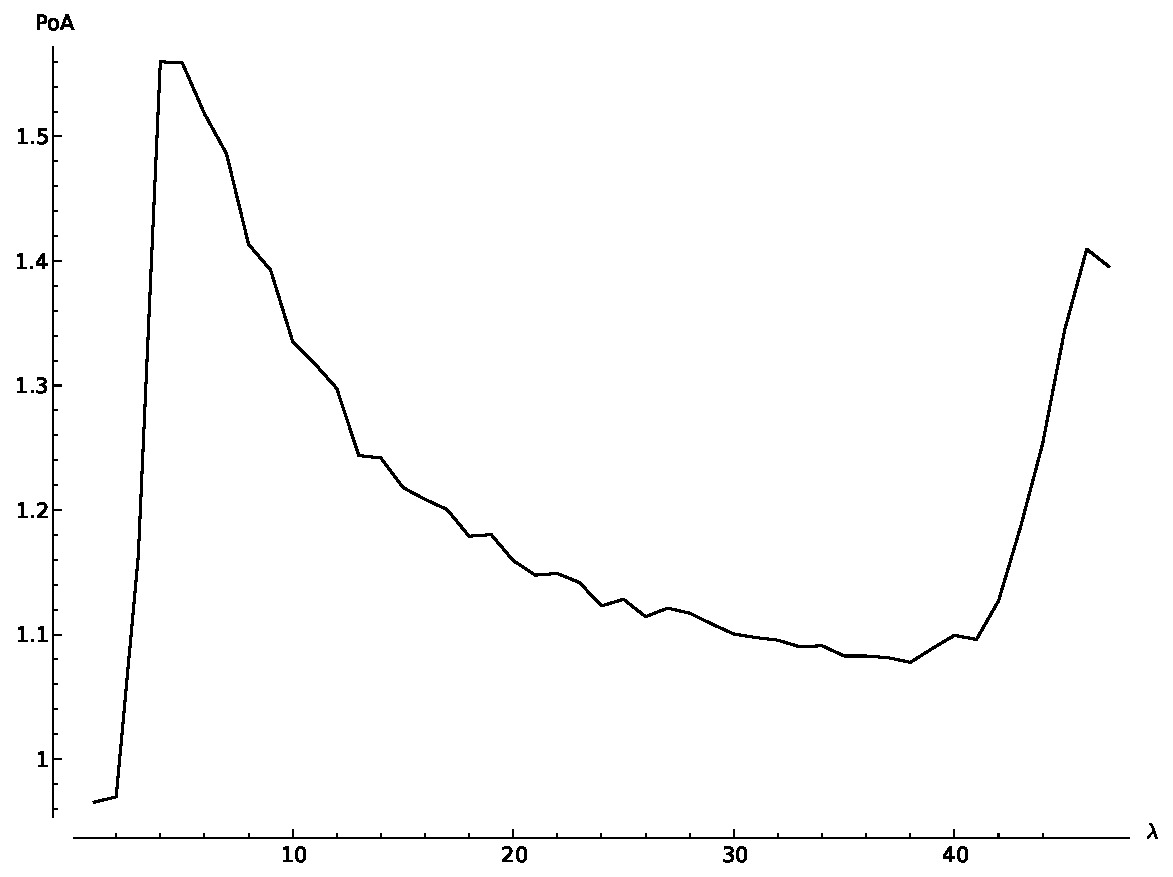
\includegraphics[width=.6\textwidth]{Images/DualPeak.pdf}
    \end{center}
    \caption{Another set of scenarios}\label{dualpeak}
\end{figure}

\section{Conclusions and Further work}\label{conclusions}

In this work ...

Note that further to understanding the effect of queues in series this work can offer some indication as to best practice by GPs.
In Figure \ref{anaexit} the PoA for the systems considered is shown for varying values of $p$ for a value of $\Lambda=$ JASON WHAT IS THIS VALUE?
The effect of selfish behaviour is reduced for a low $p$ value.
This in turn would imply that GPs would have to refer 70\% of patients to reduce the effect of selfish behaviour.
Importantly this would imply a much busier ED and an overall inefficient system however it is worth noting that measures could be put in place to counteract selfish actions although these would be quite drastic.

\begin{figure}[!hbtp]
    \begin{center}
        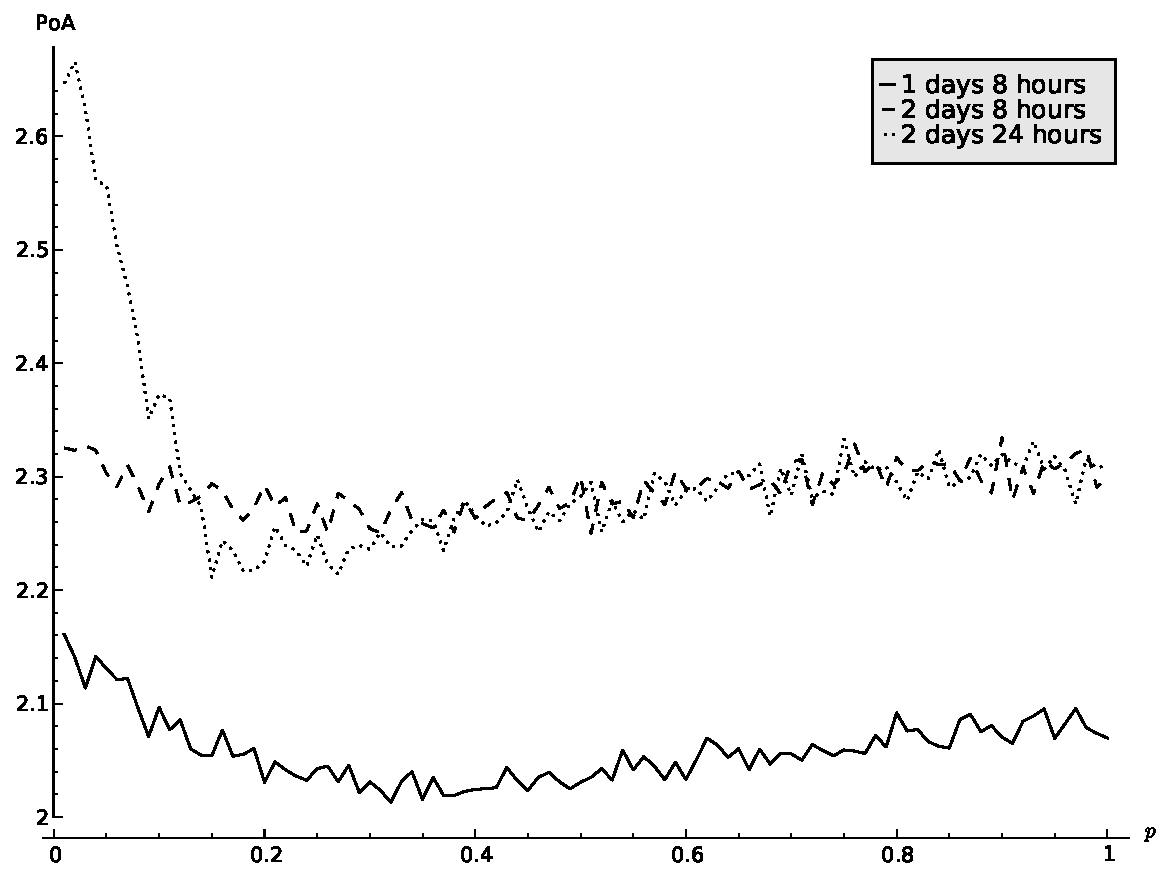
\includegraphics[width=.6\textwidth]{Images/AnaExit.pdf}
    \end{center}
    \caption{PoA for varying exit prob}\label{anaexit}
\end{figure}

Further work:

\begin{itemize}
    \item MDP
    \item Single decision
    \item Mixture of player types
\end{itemize}

\pagebreak
\bibliographystyle{plain}
\bibliography{bibliography.bib}

\end{document}
